\subsection{LED-Matrix ansteuern}
\label{subsec:ledMatrix}
In dieser Sektion soll nun eine \emph{8x8 Button-Matrix} erstellt werden, die die \emph{8x8
LED-Matrix} auf dem Sensehat des Raspberry Pi repräsentieren soll. Dabei soll der vorhandene
Joystick auf dem Sensehat dazu genutzt werden, um über die Button-Matrix zu navigieren und die
LED zu platzieren.
\newline
\newline
Da Blazor die \emph{Razor-Syntax} verwendet, kann jegliche C\# Kontrollstruktur im
\emph{HTML-Markup} verwendet werden. So kann dies auch wie folgt genutzt werden, um die \emph{8x8
Button-Matrix} zu erzeugen:

\begin{lstlisting}[language={[Sharp]C}, caption=Button-Matrix,
    label=lst:ButtonMatrix]
<div class="divGrid">
    @for (var y = 0; y < LengthY; y++)
    {
        @for (var x = 0; x < LengthX; x++)
        {
            int copyY = y;
            int copyX = x;
            <Button class="buttonBox @classes[copyY,copyX]"/>
        }
    }
</div>
\end{lstlisting}

Das \emph{@classes} Element ist ein Zwei-Dimensional Array aus Strings, mit der
Css-Klassen hinzugefügt und wieder gelöscht werden sollen. Um zu ermitteln, welcher
Joystick-Button betätigt wurde, soll ein weiterer
\emph{Timer} zum Einsatz kommen. Dieser Timer soll alle 15 Millisekunden ausgelöst werden.

\begin{lstlisting}[language={[Sharp]C}, caption=Timer: ButtonTimer,
    label=lst:ButtonTimer]
    private void StartTimer()
    {
        // More Code

        _setButtonTimer = new(15);
        _setButtonTimer.Elapsed += WriteStateToChannel;
        _setButtonTimer.Enabled = true;
    }


    private async void WriteStateToChannel(Object source, System.Timers.ElapsedEventArgs e)
    {
        if((ticks - lastTicks) > 9){
            _senseHat.ReadJoystickState();
            if(_senseHat.HoldingButton){
                await _stateChannel.Writer.WriteAsync(JoystickState.Holding);
            }
            else if(_senseHat.HoldingUp){
                await _stateChannel.Writer.WriteAsync(JoystickState.Up);
            }
            else if(_senseHat.HoldingDown){
                await _stateChannel.Writer.WriteAsync(JoystickState.Down);
            }
            else if(_senseHat.HoldingLeft){
                await _stateChannel.Writer.WriteAsync(JoystickState.Left);
            }
            else if(_senseHat.HoldingRight){
                await _stateChannel.Writer.WriteAsync(JoystickState.Right);
            }
            lastTicks = ticks;
        }
        ticks++;
    }
\end{lstlisting}

Bei \emph{JoystickState} handelt es sich um ein Enum, welches den \emph{State} des Joysticks
repräsentieren soll. Wie zu sehen ist, wird der aktuelle \emph{State} des Joysticks gelesen um,
dann das Ergebnis in einen \emph{Channel} zu schreiben.
\newline
\newline
Für die Verarbeitung des \emph{States}, wird in \emph{OnInitializedAsync} ein Task gestartet, der
in einer Endlosen schleife läuft und darauf warte bis etwas in den \emph{Channel} hinzugefügt
wurde. Sobald sich der \emph{State} geändert hat, wird entweder die Position berechnet oder
die LED an dieser Position neu eingefärbt.

\begin{lstlisting}[language={[Sharp]C}, caption=Task zum Verarbeiten des States,
    label=lst:StateTask]
        _setButtonTask = Task.Run(async () =>
        {
            while (true)
            {
                if(cancellationToken.IsCancellationRequested)
                    cancellationToken.ThrowIfCancellationRequested();
                var state = await _stateChannel.Reader.ReadAsync();
                int x = 0;
                int y = 0;
                if(state == JoystickState.Holding){
                    SetButtonBackground(_currentX, _currentY);
                }
                else if(state == JoystickState.Up){
                    y--;
                }
                else if(state == JoystickState.Down){
                    y++;
                }
                else if(state == JoystickState.Left){
                    x--;
                }else if(state == JoystickState.Right){
                    x++;
                }
                SetPositions(x, y);
                RemoveButtonBorder(_previousX, _previousY);
                SetButtonBorder(_currentX, _currentY);
                await InvokeAsync(StateHasChanged);
            }
        });

    private void SetButtonBackground(int x, int y)
    {
        if (classes[y, x].Contains(" setBackground"))
        {
            _senseHat.SetPixel(x, y, Color.Blue);
            classes[y, x] = classes[y, x].Replace(" setBackground", string.Empty);
        }
        else
        {
            _senseHat.SetPixel(x, y, Color.Red);
            classes[y, x] += " setBackground";
        }
    }
\end{lstlisting}

Wie zu sehen ist, wird die LED und der Button je
nach vorherigem Zustand entweder Blau oder Rot. Die komplette Anwendung sieht dann wie folgt aus:

\begin{figure}[h]
    \centering
    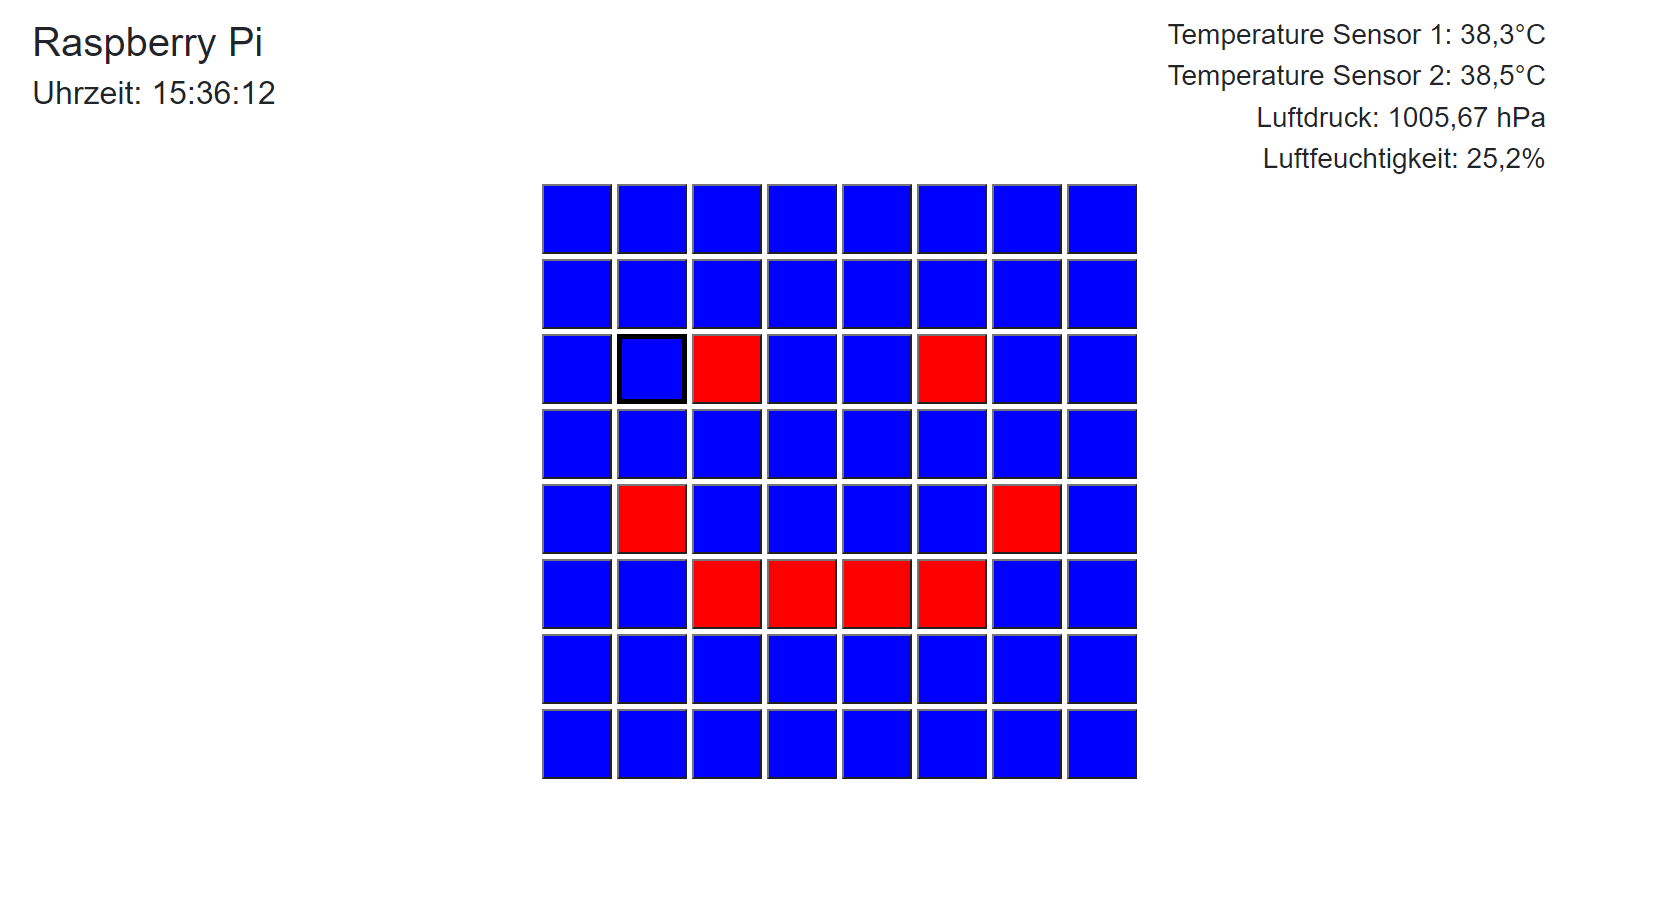
\includegraphics[width=\textwidth, center]{BlazorRasp/Demo}
    \caption[Blazor Demo]{Blazor Demo}
    \label{img:BlazorDatenAnzeigen}
\end{figure}

Da nur technisch relevante Code Abschnitte in diesem Kapitel präsentiert wurden, ist der
komplette Code im Anhang \ref{lst:DemoCode} zu finden.